\chapter{绪论}
\section{课题来源与意义}

随着大数据时代的到来,互联网数据量呈现指数上升趋势。据国际数据公司(International Data Corp, IDC)的统计和预测,2011年全球网络数据量已达到1.8ZB($ 1.8\times10^6 $TB),预计到2025年数据总量将会继续增大50倍。数据的指数级增长使学者开始关注如何从海量的数据中提取有用知识,这也是大数据分析的关键所在。2012年Google提出知识图谱(Knowledge Graph)概念,并迅速在学术界和工业界普及。基于图结构存储数据的思想普及使最终出现了很多高质量知识库,包括:DBPedia~\upcite{auer2007dbpedia,zaveri2013user}、Yago~\upcite{suchanek2007yago,hoffart2013yago2,mahdisoltani2013yago3}、Wikidata~\upcite{vrandevcic2014wikidata}、Microsoft Concept Graph\footnote{https://concept.research.microsoft.com/}等大型结构化知识库。因此如何利用现有知识库抽取有意义知识受到了广泛关注。

本文旨在利用上下位关系知识库抽取代表性话题。具体来讲就是对于给定学科领域自动抽取最具代表性的$ k $个子领域。该问题对于学生、学者、企业、政府等都具有重要意义。对于刚进入某一研究领域的学生而言,一个需要明确的问题是当前的研究热门子领域是什么、各子领域的研究热点问题是什么。本文给出的代表性子领域可以帮助学生明确研究目标,明确研究方向;对于学者而言,可以帮助明确当前的研究热点,并辅助学者寻找潜在优良研究点。比如对于机器学习(Machine learning)与医疗卫生(Health care)领域的交叉学科。可以根据历史数据得到这两个交叉学科的5个子领域之间的论文研究趋势,从而判断增长较快的研究点、研究较少的研究点。对于后者,可以分析是由于没有找到合适的方法研究还是未被人关注到,进而确定潜在研究点;对于企业而言,可以推广本文研究,进而构建噪音较少的知识图谱,进而达到更好的应用效果;对于政府而言,研究经费的分配一直是难以确定的问题。本文研究成果可用于找到目前领域内研究重点,进而帮助政府决定研究经费的分配方法。当前学者对文档话题抽取问题进行了大量研究,但是鲜有领域话题抽取的研究。

但是算法抽取的代表性话题并不一定完全符合用户的需求,因此引入用户反馈来改进模型效果是模型的关键一步,同时领域发展情况可以通过用户的反馈体现出来。因此本文希望利用强化学习的方法将用户反馈引入模型,改善模型结果。


\section{国内外研究现状}
本文旨在基于现有知识库抽取领域内代表性话题,并利用用户反馈,应用强化学习方法改进模型结果。下面首先介绍单一上下位关系的可用知识库,然后从问题定义、代表性话题抽取研究、强化学习在NLP领域的应用三个角度介绍目前国内外研究现状。

\subsection{上下位关系知识库简介}
本文研究问题主要是上下位关系抽取,因此下面将介绍三个单关系知识库:Wiki category~\upcite{ponzetto2008wikitaxonomy},ACM CCS classification tree~\upcite{coulter1998computing},以及Microsoft Field of Study~\upcite{sinha2015overview}。

Wiki category是利用维基百科数据得到的taxonomy数据集,表示上下位词之间的分类关系。通过数据处理得到一个类似树状结构。之所以说类似树,是以为其中存在少量环路,这是数据存在的问题,因此数据表现为图结构。理论上上下位关系应该是明确的,不应存在环路等情况。经过数据预处理后,可以得到一个由6,641,759个实体组成的层次结构。该结构按照维基百科的category数据给出上下位关系。比如Machine Learning的下位词数据如图\ref{fig:ml_cat}所示\footnote{https://en.wikipedia.org/wiki/Category:Machine\_learning}。
\begin{figure}
	\centering
	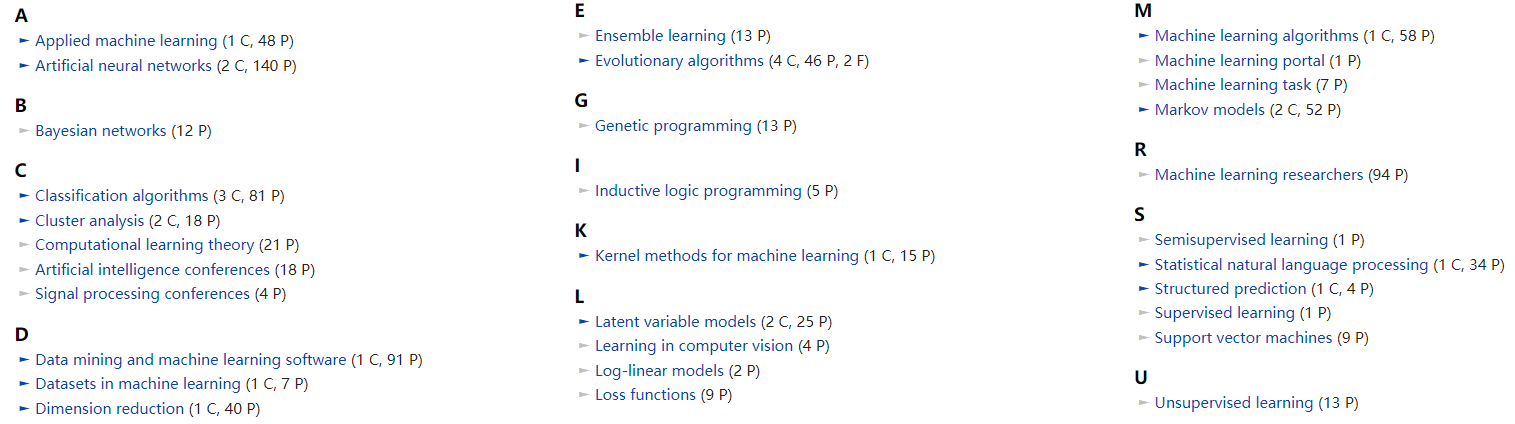
\includegraphics[width=.85\linewidth]{./figures/ml_cat.jpg}
	\caption{维基百科中Machine Learning的下位词信息}
	\label{fig:ml_cat}
\end{figure}

为说明taxonomy结构出存在的异常情况,本文给出一个三层taxonomy结构示意图,如图\ref{fig:category}所示。
\begin{figure}
	\centering
	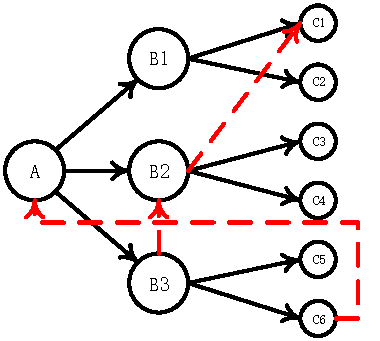
\includegraphics[width=.65\linewidth]{./figures/category.pdf}
	\caption{维基百科taxonomy层次化示意图}
	\label{fig:category}
\end{figure}

图\ref{fig:category}中红色虚线表示需要说明的情况。

\begin{enumerate}[label=\arabic*)]
	\item \textbf{B2$\rightarrow$C1}: 该路径目的是说明一个下位词可能存在多个上位词,该情况是合理的,比如一个学科可能在多个领域都有被研究。
	\item \textbf{B3$\rightarrow$B2}: 该路径说明可能兄弟之间存在上下位关系。该情况也是合理的,比如可以认为“人工智能”的两个下位词是“机器学习”和“深度学习”,而“深度学习”也可以认为是“机器学习”的下位词。
	\item \textbf{C6$\rightarrow$A}: 该路径表示出现环路,即下位词是其上位词路径上的上位词。这个显然不合理,因为上下位关系本身是一种有向关系,是一种不可逆的关系,而该路径的出现表示上下位关系可逆,因此从逻辑上讲该路径是异常的。维基百科得到的taxonomy数据存在这种关系,说明维基百科的数据在上下位关系上是存在噪声的。
\end{enumerate}


经过上述分析可知,正确上下位关系图的基本结构应为有向无环图(Directed Acyclic Graph, DAG)。

ACM CCS (Computing Classification System)分类树[8]是一个包含2126个节点的层次化实体关系,每个点可以看作一个上位词或下位词。每个非叶子节点都可作为上位词,并且在CCS分类树上存在下位词。该系统主要用于学者在ACM电子数据库中搜索符合自己需求的文献内容。同时支持将个人文章对应到CCS分类下。ACM CCS存在14个顶层分类,包括比如“Hardware”、“Network”、“Software and its engineering”等。层次深度最深达到4层。层次化数据呈现树状结构。该知识库优点是对于数据经过人工审查,分类较为仔细,缺点是只针对计算机领域,并不包括其他领域层次化数据,同时CCS发布时间是2012年,数据量过少,不包括比如“deep learning”等热门领域。因此是一个针对计算机领域的较为准确的数据库。

Microsoft Field of Study来自微软学术图(Microsoft Academic Graph, MAG)。Field of Study是微软学术图内置的一个学术上下位词关系的知识库。包含将近50000个节点,每个节点表示一个学术话题。该知识库是一个4层的有向无环图结构,每个下位词可以属于不同的上位词,MAG对这种情况给出了“可信度”这一指标,表示该下位词以多少“可信度”属于上位词。比如第3层节点“Supercomputer”是第2层节点“Operating system”的“可信度”是0.53,是第2层节点“Parallel Computing”的“可信度”是0.47。直觉上讲,超级计算机确实既会被操作系统领域研究,也会被用于并行计算研究。但是都是属于计算机领域的,因此可用Field of Study的数据得到“Supercomputer”是“Computer Science”的下位词的“可信度”是1.0。MAG的Field of Study具有严格的层次结构,它将每个节点(话题)都分成了L0至 L3这4个等级。其中L0是最高级别的上位词。统计可得各个等级的话题个数,如表\ref{tab:fos_statistics}所示。

\begin{table}[!ht]
	\centering
	\caption{MAG中Field of Study数据统计表\label{tab:fos_statistics}}
	\begin{tabular}{ccc}
		\toprule
		等级   & 个数&示例\\ \midrule
		L0 & 19 & Chemistry, Computer Science, Physics \\
		L1 & 290 & Artificial Intelligence, Organic chemistry, Algebra \\
		L2 & 1495 & Robotics, Artificial neural network, deep learning \\
		L3 & 46851 & Cognitive robotics, Logistic function, Boltzmann machine \\
		\bottomrule
	\end{tabular}
\end{table}

可以看出,L0层次的话题级别都是学科级别的话题,比如化学、计算机、物理等;L3层次的话题较为具体,一般为具体的方法等。比如logistic函数、波兹曼机等。该知识库实体个数大于ACM CCS,同时包括针对多种学科的上下位关系,不只局限于计算机领域。

以上介绍了几个常用的大规模开放可下载的知识库。同时针对本文所研究问题,介绍了3种存在上下位关系的知识库及优缺点,为了充分利用现有知识库,本文对Wiki, ACM CCS和Microsoft Field of Study进行融合,得到更大而全的上下位关系知识库。


\subsection{问题定义}

Tang等人~\upcite{tang2015sampling}从大规模社交网络中采样有代表性用户,并对问题进行了形式化定义。其中问题实例如图\ref{fig:tang_sample}所示~\upcite{tang2015sampling}。
\begin{figure}
	\centering
	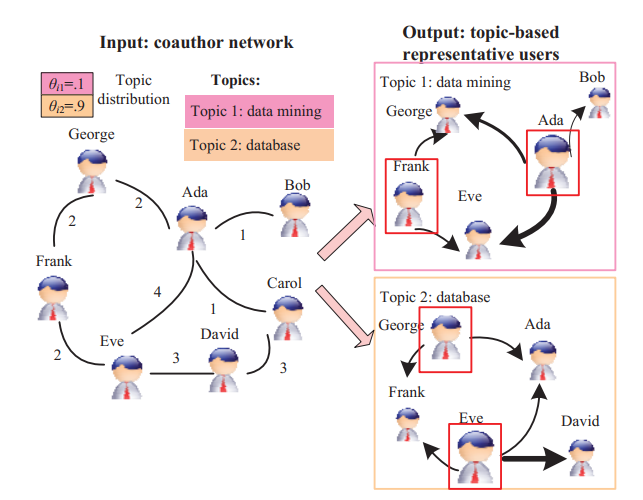
\includegraphics[width=.85\linewidth]{./figures/tang_sample.png}
	\caption{从合著者网络中采样代表性用户实例}
	\label{fig:tang_sample}
\end{figure}

对于代表性用户采样问题,给出一个社交网络$G=(V,E)$,其中$V$表示用户集合, 表示$E$有向边集合;每个用户定义有$d$个属性;希望在$V$中选出$k$个用户;将属性分为$t$组;质量函数定义为$Q$;Tang等人将如何寻找代表性用户集合$T$定义为优化问题,如式\ref{equ:tang_sample}所示:
\begin{equation}
\label{equ:tang_sample}
\setlength{\abovedisplayskip}{10pt}
\setlength{\belowdisplayskip}{10pt}
\mathop{\arg \max}_{T\subseteq V,|T=k|}{Q(G,X,\textbf{G},T)}
\end{equation}

其中$\textbf{G}$为属性组,$X$为属性的分布。$X_i$表示用户$v_i\subseteq V$的属性集合,即$X_i=[x_{ik}]_{k=1,...,d}$。

然后作者通过将问题规约为支撑集问题(Dominating Set Problem)~\upcite{garey1979guide},证明原优化问题为NP Hard问题。

\subsection{代表性话题抽取研究}

目前主要的代表性话题抽取方法包括主题模型(Topic model)、关键词抽取(Keyphrase extraction)、基于词向量的研究。

对于主题模型,可将话题看作主题模型的主题。目前主题模型已经被大量应用于抽取关键话题。Blei等人提出LDA主题模型~\upcite{blei2003latent},该模型是一种无监督学习模型,核心思想是每个文档都有多个主题混合组成,而每个单词出现在主题中的概率也不同,主题概率提供了对文档的显式表示。但是LDA模型很难给出每个分布表示的具体主题,需要通过大量人工标注。对于该问题,Mei等人提出将自动标注问题转化为最小化单词分布间的KL散度和最大化标签和主题模型的交互信息的问题。通过试验比较,发现该算法可以高效生成可解释的标签~\upcite{mei2007automatic}。Lau等人针对LDA模型提出自动标注话题的方法~\upcite{lau2011automatic}。作者利用英文维基百科数据生成标签候选集,然后利用监督学习模型SVR得出候选集标签排序,进而实现对话题的自动标注。尽管多位学者对LDA话题自动标注进行大量研究并取得一定进展,但是自动标注效果与人工标注存在明显差距。

关键词抽取技术目前主要是两种途径:监督学习和无监督学习。对于监督学习来讲,关键词抽取问题通常被看作分类问题或排序问题。Witten等人提出Kea算法用于从文本中自动抽取关键词。Kea将关键词抽取问题转化为分类问题,通过使用已知关键词的文档作为训练集,使用训练的模型找出各候选词是否属于当前文档的关键词,进而完成关键词抽取工作~\upcite{witten2005kea}。Jiang等人认为该问题类似于将候选关键词集合按特征进行排序,排名越靠前说明该关键词对于文档更重要,更可能是文档的关键词,因此作者将关键词抽取问题视为排序问题并使用learning to rank的Ranking SVM方法完成该任务,关键词抽取效果优于传统SVM和Kea算法~\upcite{jiang2009ranking}。

对于无监督学习来讲,Hasan等人将无监督方法用于解决关键词抽取问题的方法分为四组:基于图的排序法(Graph-Based Ranking)、基于主题的聚类(Topic-Based Clustering)、同时学习(Simultaneous Learning)、语言模型(Language Modeling)~~\upcite{hasan2014automatic}。

基于图的排序法最有代表性的是Kleinberg等人提出的HITS算法~\upcite{kleinberg1999authoritative}和Google提出的PageRank算法~\upcite{brin1998anatomy}。Mihalcea等人提出TextRank算法用于自动关键词抽取~\upcite{mihalcea2004textrank},将文本看成图,将本文分词,并进行词性标注,用点表示关键词,边表示关键词之间的共现关系构成图。基于PageRank算法思想,迭代计算各节点权重,直到收敛。根据迭代结果找出最重要的 个单词,即为关键词。

基于主题的聚类法是将关键词分成多个主题组,直觉上每个抽取出来的关键词应该包含文章中的所有主要主题。Liu等人利用聚类技术找出代表性术语,将每个类的代表性属于作为种子自动抽取关键词。研究表明大部分人工选取的关键词都是名词,因此作者对文档进行词性标注,主要抽取其中的名词和形容词。实验表明准确率在F1值上超过TextRank 9.5\%~\upcite{liu2009clustering}。Hasan等人指出基于关键词聚类的方法为所有主题分配相同的重要性,实际文档中有些话题并不主要~\upcite{hasan2014automatic},因此可能存在缺陷。

同时学习是基于一个假设:重要的词出现在重要的句子中,重要的句子包含重要的词。因此文本摘要和关键词抽取同时学习可能能共同提高效果~\upcite{zha2002generic}。Wan等人进一步做出两点假设:1)关键句与其他关键句相连;2)关键词与其他关键词相连~\upcite{wan2007towards}。基于上述假设,Wan等人寄建立三个捕获句子(S)和单词(W)间关系的图:S-S图、S-W图和W-W图。S-S图的边权重表示两个句子的相似度;S-W图的边权重表示词在句子中的重要性;W-W图的边权重表示两个单词之间的共现次数或者基于知识的相似度。最后通过迭代强化算法为每个句子和单词分配权重,权重高的单词作为关键词~\upcite{wan2007towards}。

语言模型通过两个特征评价关键词:词组性(Phraseness)和信息性(Informativeness)~\upcite{tomokiyo2003language}。词组性表示单词序列是否可看作词组;信息性表示哪个单词捕获了文档的中心含义。直觉上讲,有高词组性和信息性的词组更可能是关键词。Tomokiyo等人通过语言模型分别在前景语料库(Foreground corpus)和背景语料库(Background corpus)上训练得到这两个特征。前景语料库由存在关键词的文档组成,背景语料库是来自Web的大量无标注文本数据。通过语言模型得到特征值之后按照两者加和排序候选关键词~\upcite{tomokiyo2003language}。

词向量(Word Embedding)将单词特征进行稠密编码,将特征映射到隐特征空间。Mikolov等人提出通过预测单词和上下文单词来获取低维特征表示的Word2Vec方法~\upcite{mikolov2013distributed}。Word2Vec的主要包括两种算法:Skip-gram(SG)和连续词袋模型(Continuous Bag of Words, CBOW)。SG算法是通过当前单词预测上下文单词,CBOW是通过上下文单词的词袋模型预测目标单词。训练时为了更加高效可以使用两种算法:层次化Softmax(Hierarchical Softmax)和负采样(Negative Sampling)。因为本文研究是基于词向量相似度的代表性话题抽取,因此下面重点介绍Skip-gram模型的工作流程。

Skip-gram模型通过当前单词预测周围单词出现的概率。如图\ref{fig:skip_gram_model}所示~\upcite{mikolov2013distributed}。
\begin{figure}
	\centering
	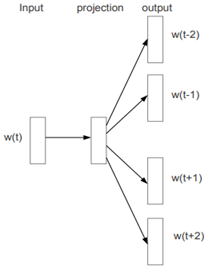
\includegraphics[width=.45\linewidth]{./figures/skip_gram_model.png}
	\caption{Skip-gram模型结构}
	\label{fig:skip_gram_model}
\end{figure}

Skip-gram通过单隐层神经网络完成预测周围单词出现概率的任务。但这实际是一个“伪任务”~\upcite{mccormick2016word2vec}。即真正想要的并不会真正使用模型去完成上述预测任务,而是为了得到隐层权重,因此实际“伪任务”得到的权重就是通过Skip-gram模型得到的词向量。

输出的概率表示每个单词更有可能在输入单词附近的概率。比如给出输入单词“Soviet”,周围的单词是“Union”或者“Russia”的概率较大,而是“西瓜”或者“袋鼠”的概率就很小~\upcite{mccormick2016word2vec}。而在输入单词附近由“窗口大小”衡量。比如存在句子“The quick brown fox jumps over the lazy dog.”,假设窗口大小$c=2$。表示在中心词前后各选择两个单词作为环境词。最终得到训练样本<输入,输出>为:<the, quick>, <the, brown>, <quick, the>, <quick, brown>, <quick, fox>, <brown, the>, <brown, quick>, <brown, fox>, <brown, jumps>, <fox, quick>, <fox, brown>……后面模式相同。通过训练,即可通过训练好的模型预测当前单词周围的词汇出现的概率。

更一般地,给出句子序列$S=<w_1,w_2,...,w_T>$,其中$T$为序列长度。利用最大似然估计可得,Skip-gram的目标是最大化式:
\begin{equation}
\label{equ:skip_gram_target}
\setlength{\abovedisplayskip}{10pt}
\setlength{\belowdisplayskip}{10pt}
J(\theta)=-\frac{1}{T}\sum_{t=1}^{T}\sum_{-c\leq j\leq c, j\neq 0}\log p(w_{t+j}|w_t)
\end{equation}

其中$c$是训练窗口大小,$c$越大训练数据越多,准确率也越高,但是耗费时间也越大。式\ref{equ:skip_gram_target}中的$p(w_{t+j}|w_t)$使用了softmax函数表示,如式\ref{equ:skip_gram_p}所示。
\begin{equation}
\label{equ:skip_gram_p}
\setlength{\abovedisplayskip}{10pt}
\setlength{\belowdisplayskip}{10pt}
p(w_O|w_I)=\frac{\exp ({v'_{wO}}^{T}v_{wI})}{\sum_{w=1}^{W} \exp ({v'_w}^{T}v_{wI})}
\end{equation}

其中$v_w$和$v'_w$分别表示单词$w$的输入、输出向量表示。$W$表示词表大小。

实际该模型可以展示为一个三层的神经网络。其中隐含层为线性激活单元,输出层为Softmax分类器。具体结构如图\ref{fig:skip_gram_structure}所示~\upcite{mccormick2016word2vec}。
\begin{figure}
	\centering
	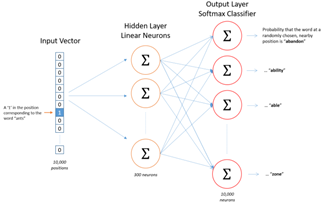
\includegraphics[width=.65\linewidth]{./figures/skip_gram_structure.jpg}
	\caption{Skip-gram网络结构示意图}
	\label{fig:skip_gram_structure}
\end{figure}

输入层到隐含层的参数$W$维度为$|V|\times |H|$,即词表大小乘以隐含层大小。$w(i,:)$可以看作第$i$个单词的词向量。如果两个不同的单词有相似的上下文,即出现在其周围的单词较为相似,则Skip-gram模型将输出相似的结果。因此如果两个单词上下文相似,则模型倾向于学习相似的词向量。

因此可知,词意相似的单词词向量也比较相似,而可以认为下位词的词向量应与上位词词向量相似,进而实现代表性话题抽取。尽管存在Glove等更优秀的单词分布式表示方法~\upcite{pennington2014glove},但是由于效率和易用性等原因,还是考虑使用Skip-gram。

\subsection{强化学习在NLP领域的应用}

近年来,强化学习(Reinforcement Learning)与深度学习结合,开始成为研究热点问题~\upcite{mnih2013playing}。因此强化学习也在各领域大放异彩。2015年10月AlphaGo击败欧洲围棋冠军,2016年3月击败18次获得世界围棋比赛冠军的李世石,2017年5月击败围棋世界第一柯洁。并且提出完全自我训练的AlphaGo~\upcite{silver2016mastering}。2017年12月,Deep Mind团队公开AlphaZero~\upcite{silver2017mastering},同时在多种棋类上做出大量提升。这是强化学习最引人注目的应用之一~\upcite{silver2016alphago}。下面本文先简单介绍强化学习的基本知识和核心概念,然后介绍近年来强化学习在NLP领域的应用。

强化学习是Agent与环境(Environment)交互的过程,通过学习最优策略(Policy)和试错(Trail and error)解决序列决策问题(Sequential decision making problem)。强化学习问题在于学习做什么才能最大化所得奖赏(Reward),即如何将当前状态(State)映射为动作(Action)。本质上强化学习问题是一个闭环问题(Closed-loop),因为学习系统的行为会影响下一次的输入~\upcite{sutton1998reinforcement}。强化学习过程示意图如图\ref{fig:rl_interaction}所示\footnote{goo.gl/UqaxlO}。

\begin{figure}
	\centering
	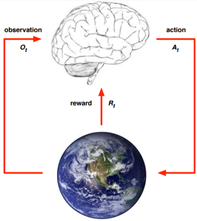
\includegraphics[width=.65\linewidth]{./figures/rl_interaction.png}
	\caption{强化学习Agent和Environment交互过程}
	\label{fig:rl_interaction}
\end{figure}

图\ref{fig:rl_interaction}展示了强化学习的交互过程,其中,在第$t$步,agent执行动作$A_t$,收到观测$O_t$等价于上文所述的State$S_t$),收到标量奖赏$R_t$。环境收到动作$A_t$,发出观测$O_{t+1}$(等价于$S_{t+1}$),发出标量奖赏$R_{t+1}$。$t$在每次交互完成后递增。

定义当前时刻$t$的累计奖赏为:
\begin{equation}
\label{equ:rl_reward}
\setlength{\abovedisplayskip}{10pt}
\setlength{\belowdisplayskip}{10pt}
R_t=\sum_{k=0}^{\infty} \gamma^kr_{t+k}
\end{equation}
其中$\gamma\in(0,1]$为折扣因子(discount factor),$r_t$表示$t$时刻的即时奖赏。

价值函数(Value Function)用于衡量当前状态的好坏程度,可用累计奖赏的期望表示。即:
\begin{equation}
\label{equ:rl_value_function}
\setlength{\abovedisplayskip}{10pt}
\setlength{\belowdisplayskip}{10pt}
v_\pi(s)=E[R_t|s_t=s]
\end{equation}
其中$v_\pi(s)$为在状态$s$下使用策略$\pi$的期望累积奖赏值。将$v_\pi(s)$分解为Bellman等式可得:
\begin{equation}
\label{equ:rl_bellman}
\setlength{\abovedisplayskip}{10pt}
\setlength{\belowdisplayskip}{10pt}
v_\pi(s)=\sum_a \pi(a|s)\sum_{s',r}p(s',r|s,a)[r+\gamma v_\pi(s')]
\end{equation}

最优状态值可定义为:
\begin{equation}
\label{equ:rl_optimal}
\setlength{\abovedisplayskip}{10pt}
\setlength{\belowdisplayskip}{10pt}
v_*(s)=\max_\pi v_\pi (s)=\max_a q_{\pi *}(s,a)
\end{equation}

若强化学习问题满足Markov性质,即下一步状态只依赖于当前状态和动作,与过去无关,则可以将问题看作Markov决策过程(Markov Decesion Process, MDP),用五元组$(S,A,P,R,\gamma)$表示~\upcite{li2017deep}。对于有模型学习(Model-based learning)问题,机器已对环境进行建模,状态、动作、状态转移概率、转移奖赏函数均为已知,则可考虑使用动态规划方法:策略评估(Policy evaluation)计算策略的价值函数,策略迭代(Policy iteration)或值迭代(Value iteration)找到最优策略。对于免模型学习(Model-free learning)问题,环境转移概率、奖赏函数、甚至不知道环境中一共有多少状态。此时可以使用蒙特卡洛方法,根据执行该策略$T$步得到的采样轨迹$<s_0,a_0,r_1,s_1,a_1,...,s_{T-1},a_{T-1},r_T,s_T>$可得到状态-动作值函数的估计。另一种解决方法是时序差分学习(Temporal Difference, TD),同时利用采样轨迹和动态规划结构,得到值函数或状态-动作值函数的估计。SARSA算法~\upcite{rummery1994line}和Q-Learning算法~\upcite{watkins1992q}是经典的TD learning算法~\upcite{arulkumaran2017brief}。

之前提到的值函数或状态-动作值函数均被以表格形式存储,但是当状态空间很大或者连续时,内存需求会太大甚至无法存储,因此需要使用近似值函数(Function Approximation)估计值函数。这种近似函数可以是线性函数或非线性函数,DQN则通过使用CNN实现端到端的强化学习~\cite{mnih2013playing,mnih2015human},实现直接从像素输入学习游戏打法并超过顶尖人类玩家水平。

除了TD learning和Q-learning等基于值的方法(Value-based methods),还有基于策略的方法(Policy-based methods)。基于策略的方法目标是直接优化策略$\pi(a|s;\theta)$,其中$\theta$是近似函数的参数,并通过梯度上升(Gradient ascent)方法优化$E[R_t]$。Williams等人提出的REINFORCE算法是一种经典策略梯度(Policy gradient)算法,在方向$\nabla_\theta \log \pi(a_t|s_t;\theta)$上更新参数$\theta$。

强化学习在多个NLP子领域开始被应用,包括对话系统(Dialogue system)、机器翻译(Machine translation)、文本生成(Text generation)~\cite{li2017deep,williams1992simple}。在对话系统领域,Li等人基于监督学习和强化学习提出端到端的神经对话系统。该框架包括用户仿真器和神经对话系统。作者利用强化学习端到端的训练系统,将对话策略看作DQN,进而降低其他模块产生的噪声~\cite{li2017end}。在机器翻译领域,He等人提出对偶学习处理机器翻译领域数据不足的问题。机器翻译从语言A到语言B和对偶任务,从语言B到语言A,可以帮助提高两个翻译模型性能。作者使用策略梯度方法,使用语言模型似然度作为奖励函数。实验表明该模型只需要较少数据即可实现优越性能~\cite{he2016dual}。文本生成是多种NLP任务的基础,比如对话生成、机器翻译、自动摘要等。Bahdanau等人使用强化学习算法actor-critic实现序列预测,使用critic网络预测单词的价值,即actor网络定义的序列预测策略的期望累计价值~\cite{bahdanau2016actor}。除此之外,强化学习开始被用于微调(Fine-tuning)模型结果。Zhang等人使用RNN decoder和attention机制对病人病症生成治疗药物,保证药物之间不出现药物冲突。使用策略梯度方法基于规则去除仍存在冲突的药物组合,实验表明强化学习可以实现机制冲突药物组合的产生~\cite{zhang2017leap}。


\section{论文研究内容}
在历史文献当中,源词和目标词分别被称为模型的输入和输出。源词通常可以用分布式表示(Distributed Representation)来表示,称为输入词嵌入(Word Embedding),通常在大规模语料上使用连续词袋模型(CBoW)、跳跃单词模型(Skipgram)或者~Fasttext~模型来训练。
而这几种模型均起源于语言建模任务,并且考虑到实际运算的效率而去除了部分冗余结构。
另外,输出端的词表通常表示为单词索引(Indexing)或~$1-K$~编码,并且可以与~softmax~概率函数直接关联。

在语言模型研究领域中,大词表问题是目前理论应用到实际过程中必须要克服的问题,我们当然可以通过配置高性能服务器来缓解该计算瓶颈。一旦应用到较大规模的数据集上,即使是目前最好的中央处理器(CPU)或者通用计算图形处理器(GPGPU),仍然需要数周时间才能训练完善。因此,在保证原有模型的准确率和精度的前提下,如何提高模型的训练速度是本文主要讨论和研究的内容。为此我们考察了两个主要的研究目标:上下文信息建模效率和精度对比、大词表问题的优化和研究。

针对大词表问题的优化,目前主要采用的方案有以下几种:一种是采用子词(Subword-level)或者字符级别的词(Character-level)来直接缩小词表大小;一种是通过采样技术(Sampling-based Approximation)来减少必要的训练时间;另一种是通过基于分类的多元分类(class-based Hierarchical Softmax,cHSM)和采用基于树模型的多层二元分类模型(tree-based Hierarchical Softmax,tHSM)来加速模型。

本论文考虑了层次概率模型所存在的一些问题,并提出相应的解决策略。首先,我们提出了一个在分层结构上建模参数的单词编码方案,推导出紧凑的代价函数及其梯度。同时考虑到类或树上的单词分布对其性能有很大的影响,我们运用文本的统计,句法和语义知识来初始化其参差结构,以达到稳定的计算精度。同时在推理过程中,我们考虑了两种不同的推理情况:句子打分和文本排序,并提出了对应的优化策略。
\section{论文的组织结构}
\textbf{第一章:}``绪论'',主要介绍了本论文的研究背景和意义,另外简要说明了语言模型的发展历史以及本文的主要工作,并对本文的组织架构进行了说明。

\textbf{第二章:}``相关技术介绍'',对历史上的各个学术分支在语言模型的任务上的相关工作进行了介绍。

\textbf{第三章:}``树状层次概率模型'',介绍了基于二叉树的层次概率模型,并与传统树状模型做了理论层面的比较。同时还研究了在推理测试阶段,二叉树层次概率模型应用的贪心策略,以保证实际测试结果性能和效率。

\textbf{第四章:}``类别层次概率模型'',介绍基于分类的层次概率模型,并分析了词表非均匀划分所产生的后果,进而探讨了类别不均匀问题所带来的影响以及相关解决策略。最后探讨了在测试阶段,语言模型的任务需求和分类层次概率模型相应的解决算法。

\textbf{第五章:}``语言建模实验及结果分析'',实证研究了本论文提出的层次概率模型的实际效果,并和其他算法在各个指标维度上进行了比较和分析。

最后结论部分,总结了全论文的贡献和工作,并提出了未来的工作方向,同时撰写了结束语。



